\documentclass[12pt,A4paper]{article}
\usepackage[utf8]{inputenc}
\usepackage[T1]{fontenc}
\usepackage{amsmath}

\usepackage{url}
\usepackage{hyperref}
\usepackage{graphicx}
\usepackage{listings}
\usepackage[usenames,dvipsnames]{color}

% This is the color used for MATLAB comments below
\definecolor{MyDarkGreen}{rgb}{0.0,0.4,0.0}

% For faster processing, load Matlab syntax for listings
\lstloadlanguages{Matlab}%
\lstset{language=Matlab,                        % Use MATLAB
        frame=single,                           % Single frame around code
        basicstyle=\small\ttfamily,             % Use small true type font
        keywordstyle=[1]\color{Blue}\bfseries,        % MATLAB functions bold and blue
        keywordstyle=[2]\color{Purple},         % MATLAB function arguments purple
        keywordstyle=[3]\color{Blue}\underbar,  % User functions underlined and blue
        identifierstyle=,                       % Nothing special about identifiers
                                                % Comments small dark green courier
        commentstyle=\usefont{T1}{pcr}{m}{sl}\color{MyDarkGreen}\small,
        stringstyle=\color{Purple},             % Strings are purple
        showstringspaces=false,                 % Don't put marks in string spaces
        tabsize=5,                              % 5 spaces per tab
        %
        %%% Put standard MATLAB functions not included in the default
        %%% language here
        morekeywords={xlim,ylim,var,alpha,factorial,poissrnd,normpdf,normcdf},
        %
        %%% Put MATLAB function parameters here
        morekeywords=[2]{on, off, interp},
        %
        %%% Put user defined functions here
        morekeywords=[3]{FindESS, homework_example},
        %
        morecomment=[l][\color{Blue}]{...},     % Line continuation (...) like blue comment
        numbers=left,                           % Line numbers on left
        firstnumber=1,                          % Line numbers start with line 1
        numberstyle=\tiny\color{Blue},          % Line numbers are blue
        stepnumber=5                            % Line numbers go in steps of 5
        }
\usepackage{float}
\usepackage{pythonhighlight}
\usepackage[export]{adjustbox}

\usepackage[margin=0.5in]{geometry}

\begin{document}
        \begin{center}
        \vspace*{1cm}    
        \Huge
        \textbf{Lab8-Report}
            
        \vspace{0.5cm}
        \LARGE
        RollNo-190020021
            
        \vspace{0.5cm}
            
        \textbf{Kushagra Khatwani}
	\end{center}
	
	\vspace{.5cm}
	
	\section*{Answers-}
	\subsection*{Q1-}
	\begin{figure}[H]
		\centering
		\colorbox{gray}{\includegraphics[height=6in]{/Users/kushagrakhatwani/Downloads/l_1.jpg}}
	\end{figure}
	\begin{figure}[H]
		\centering
		\colorbox{gray}{\includegraphics[height=9in]{/Users/kushagrakhatwani/Downloads/l_2.jpg}}
	\end{figure}
	\begin{figure}[H]
		\centering
		\colorbox{gray}{\includegraphics[height=9in]{/Users/kushagrakhatwani/Downloads/l_3.jpg}}
	\end{figure}
\begin{figure}[H]
		\centering
		\colorbox{gray}{\includegraphics[height=9in]{/Users/kushagrakhatwani/Downloads/l_4.jpg}}
	\end{figure}
\begin{figure}[H]
		\centering
		\colorbox{gray}{\includegraphics[height=6in]{/Users/kushagrakhatwani/Downloads/l_5.jpg}}
	\end{figure}
	\subsection*{Code Fragment for K=1-}
	\lstinputlisting[language=Matlab]{Q2.m}
\begin{figure}[H]
	\subsection*{Plot for K=1}
		\centering
		\colorbox{gray}{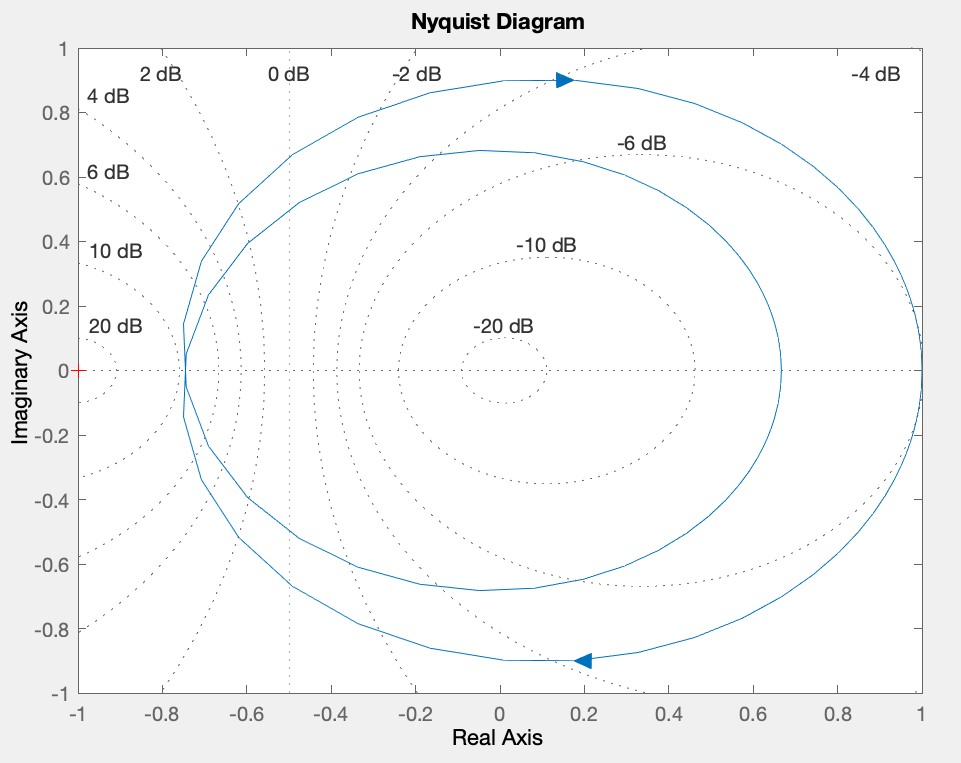
\includegraphics[height=5in]{/Users/kushagrakhatwani/Desktop/1}}
	\end{figure}
	As K<1.34 for stable system so-
		\subsection*{Simulink for K=1.25-}
	\begin{figure}[H]
		\centering
		\colorbox{gray}{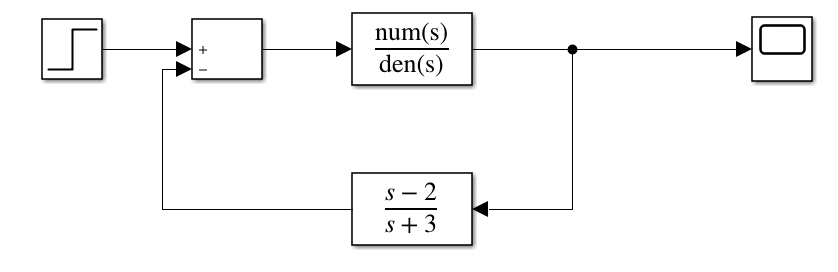
\includegraphics[height=2in]{/Users/kushagrakhatwani/Desktop/2}}
	\end{figure}
			\subsection*{Plot from scope-}
				\begin{figure}[H]
		\centering
		\colorbox{gray}{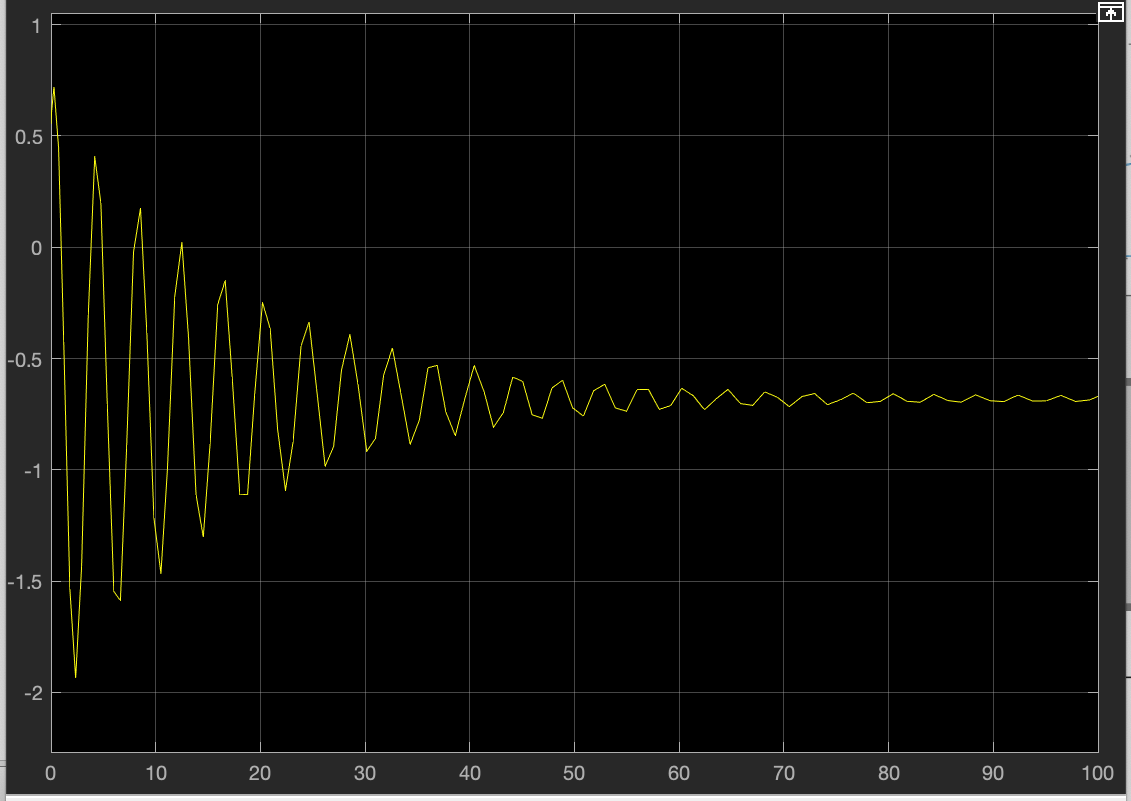
\includegraphics[height=4in]{/Users/kushagrakhatwani/Desktop/3}}
	\end{figure}
	We can see from the above plot that for controller value of K=1.25 system is stable.
	\subsection*{Code for Gain and Phase margins-}
		\subsection*{K=1000}
		\lstinputlisting[language=Matlab]{Q2_5.m}
			\subsection*{Output-}
			gain margin = -57.501231\\
 phase margin = Inf 
		\begin{figure}[H]
	\subsection*{Plot for K=1000}
		\centering
		\colorbox{gray}{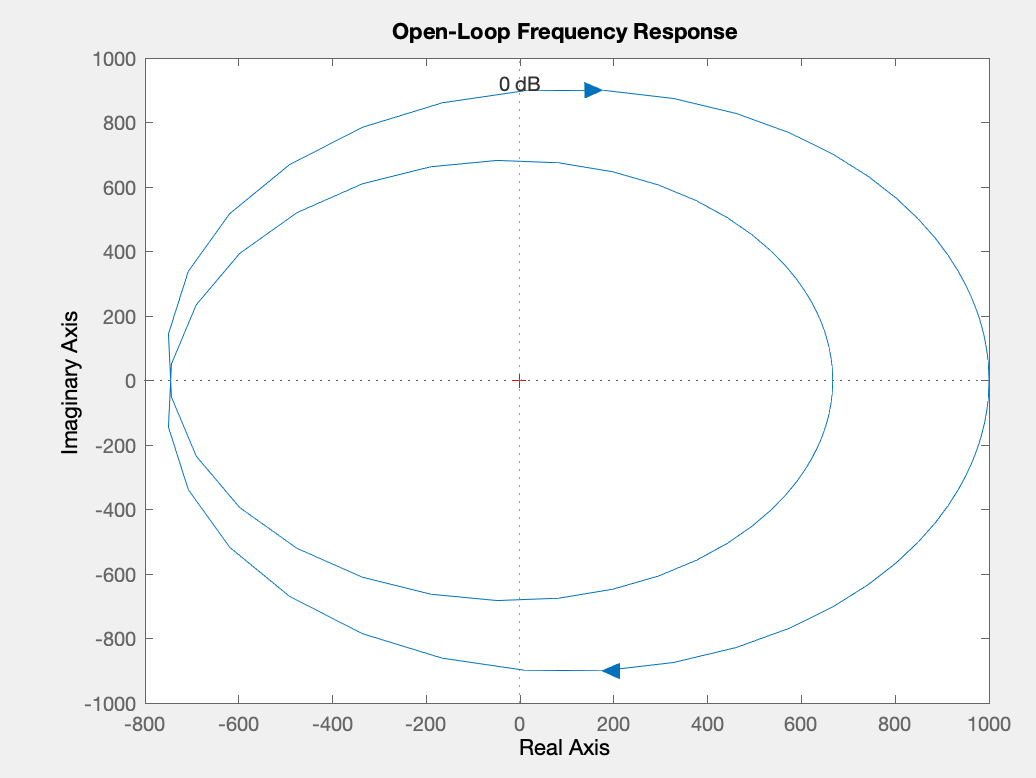
\includegraphics[height=5in]{/Users/kushagrakhatwani/Desktop/4}}
	\end{figure}
			\subsection*{K=100}
		\lstinputlisting[language=Matlab]{Q2_5_1.m}
			\subsection*{Output-}
	gain margin = -37.501231\\
 phase margin = Inf 
		\begin{figure}[H]
	\subsection*{Plot for K=100}
		\centering
		\colorbox{gray}{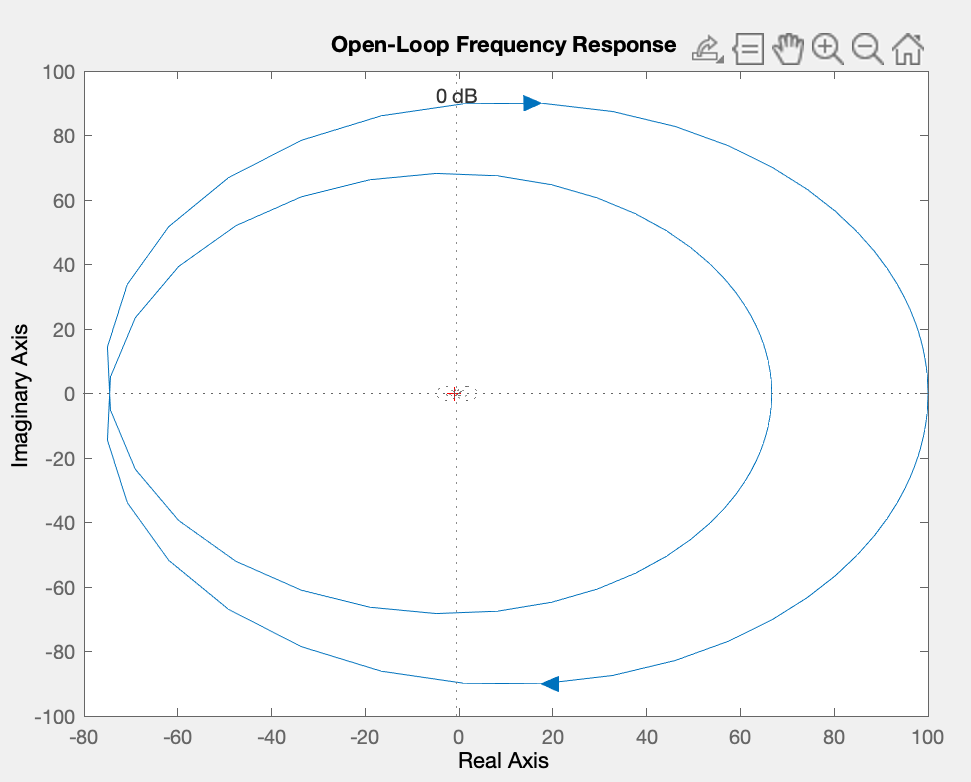
\includegraphics[height=5in]{/Users/kushagrakhatwani/Desktop/5}}
	\end{figure}
			\subsection*{K=0.1}
		\lstinputlisting[language=Matlab]{Q2_5_2.m}
			\subsection*{Output-}
gain margin = 22.498769
 phase margin = Inf 
		\begin{figure}[H]
	\subsection*{Plot for K=0.1}
		\centering
		\colorbox{gray}{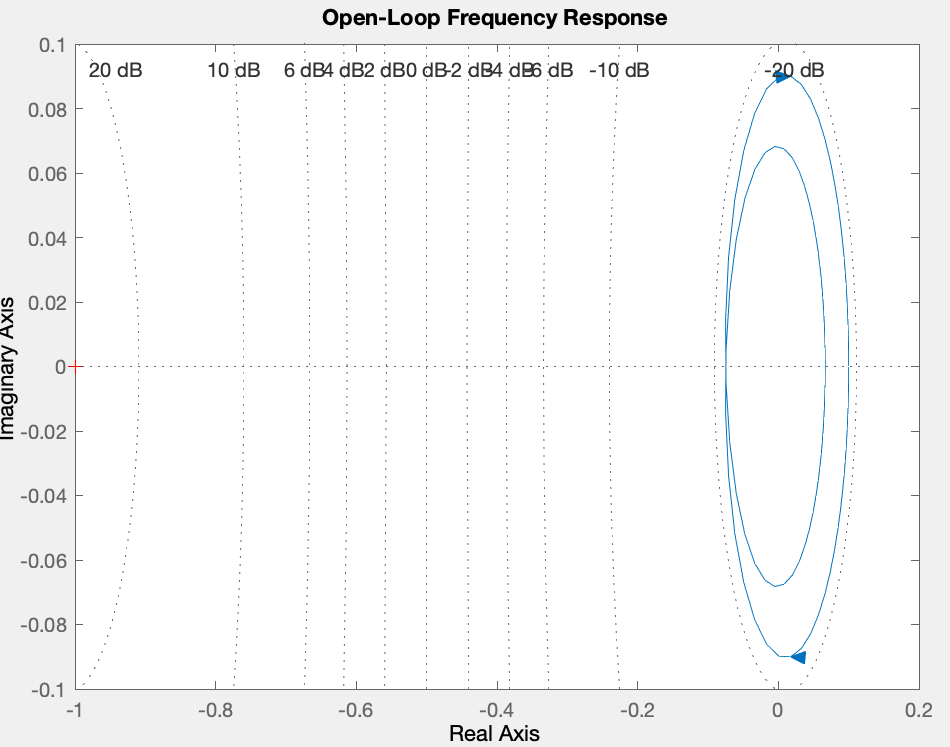
\includegraphics[height=5in]{/Users/kushagrakhatwani/Desktop/6}}
	\end{figure}
	Extra Problems on next page.
	\section*{Extra Problems Answers-}
	\subsection*{Q1-}
	\begin{figure}[H]
		\centering
		\colorbox{gray}{\includegraphics[height=9in]{/Users/kushagrakhatwani/Downloads/m_1.jpg}}
	\end{figure}
	\begin{figure}[H]
		\centering
		\colorbox{gray}{\includegraphics[height=9in]{/Users/kushagrakhatwani/Downloads/m_2.jpg}}
	\end{figure}
	\begin{figure}[H]
		\centering
		\colorbox{gray}{\includegraphics[height=6in]{/Users/kushagrakhatwani/Downloads/m_3.jpg}}
	\end{figure}
	\subsection*{Q2-}
	\begin{figure}[H]
		\centering
		\colorbox{gray}{\includegraphics[height=9in]{/Users/kushagrakhatwani/Downloads/m_4.jpg}}
	\end{figure}
\end{document}
	